\documentclass[english]{article}
\usepackage[T1]{fontenc}
\usepackage[utf8]{inputenc}

\usepackage{babel}
\usepackage{authblk}
\usepackage{xspace}
\usepackage{graphicx,graphics} 
\usepackage{color}
\usepackage{amsmath}
\usepackage{amsfonts}
\usepackage{algorithm}
\usepackage{algorithmic}
\usepackage{amssymb}
\usepackage{amsthm}
\usepackage{algorithm}
\usepackage{algorithmic}
\usepackage{longtable}
\usepackage{complexity}
\usepackage{hyperref}
\usepackage{tkz-graph}
\begin{document}

\title{Scheduling algorithm to avoid contention in meshed networks}
 

\newcommand{\todo}[1]{{\color{red} TODO: {#1}}}
\newcommand{\spall}{\textsc{SPALL}\xspace}
\newtheorem{theorem}{Theorem}
\newtheorem{lemma}[theorem]{Lemma}
\newtheorem{definition}{Definition}
\newtheorem{corollary}{Corollary}
\author[1]{\bf{ {Dominique Barth}}}
\author[1,2]{\bf{ {Ma\"el Guiraud}}}
\author[2]{\bf{ {Brice Leclerc}}}
\author[2]{\bf{ {Olivier Marc\'e}}}
\author[1]{\bf{ {Yann Strozecki}}}


\affil[1]{David Laboratory, UVSQ}
\affil[2]{Nokia Bell Labs France}


\maketitle

\section*{Introduction}

TODO: doner le contexte CRAN, puis l'objectif d'optimisation de latence. 
Dire qu'on a déjà fait désynchronysé mais que dans les archtectures actuelles il faut plutot faire synchronisé.
Comparer à nos travaux antérieurs et à d'autres qu'on a déjà cité (voir les papiers précédents, surtout les citations du dernier)




\section{Modeling Periodic Scheduling of datagrams over a Network}


Let $[n]$ denote the interval of $n$ integers $\{0,\dots,n-1\}$.

  \subsection{Modeling the Networks and its Contention Points}

  We study a communication network with pairs of source-destination nodes between which messages are sent periodically. The routing between each  pair of such nodes is given. The network is represented by a directed acyclic multigraph $G=(V,A)$. The set of vertices is composed of three disjoint subsets:  ${\cal S}$ the set of sources of the messages, ${\cal D}$ the set of destination of the messages, and ${\cal C}$ the set of contention points in the network. Indeed, some links of the network are shared between several pairs of source-destination nodes. A contention point represent the beginning of a shared link, i.e. the physical node of the network which sends the messages into the link. An arc in $G$ can represent several physical links or nodes, which do not induce contention points. Each arc  $(u,v)$ in $A$ is labeled by an integer weight $\omega(u,v)$ which represents the number of tics elapsed between the sending time of the message in $u$ and the reception time of this message in $v$ using this arc. \\
  A {\bf route} $r$ in $G$ is a directed path, that is, a sequence of adjacent vertices $u_1, \ldots , u_{l}$, with $(u_i,u_{i+1}) \in A$.  The {\bf weight of a vertex} $u_i$ in a route $r=(u_0,\dots,u_l)$ is defined by $\lambda(u_i,r)= \sum\limits_{1 \leq j <i} \omega(u_j, u_{j+1})$. It is the number of tics needed by a message to go from the first vertex of the route to $u_i$. The \textbf{length} of the route $r$ is defined by $\lambda (r)= \lambda (u_l,r)$.
	We denote by ${\cal R}$ a set of routes of the graph $G$, the pair $(G,{\cal R})$ is called a \textbf{routed network} and represents our telecommunication network.\\
	Let $r \in {\cal R}$, with $r = (u_0,u_1,\dots,u_l)$, then we say that $u_i$ is of \textbf{contention level} $i$ for the route $r$, and we denote it by $cl(u_i,r) = i$. The contention level of a node $u$ is the maximum of its contention level over all routes going through itself: 
	$cl(u) = \max\limits_{r\in{\cal R} \text{ and } u \in r} cl(u,r)$.

	\begin{figure}[h]
	\centering
	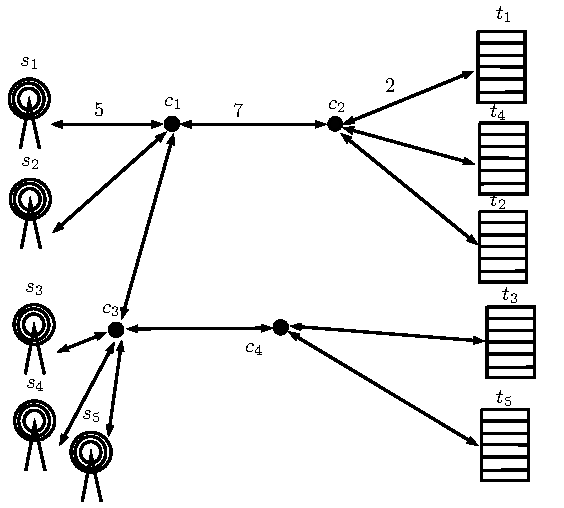
\includegraphics[scale=0.5]{fronthaul}
\caption{A C-RAN fronthaul network}
\label{fig:fronthaul}
\end{figure}
	\begin{figure}[h]
	\centering
	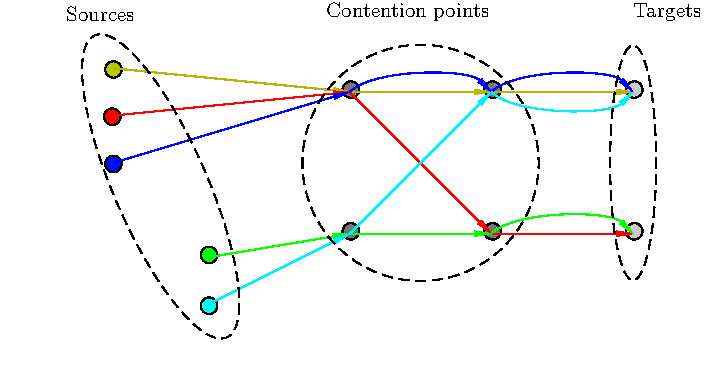
\includegraphics[scale=0.5]{graphmodel}
\caption{The corresponding routed network }
\label{fig:graph}
\end{figure}
	The  \textbf{contention depth} of a routed network $(G,{\cal R})$ is equal to the maximum of the contention level over all vertices. It is the number of contention points on the longest route of the network. In all the article, $(G,{\cal R})$ is the routed network, the number of routes, $|\cal{R}|$, is denoted by $n$ and the contention depth is denoted by $d$. The set ${\cal C}$ denotes the set of contention vertices.


 \subsection{Datagram Transmission over the Network}
	    
 		In this article, we consider a discretized time. The unit of time is called a {\bf tic}. This is the time needed to send an atomic data in a link of the network. We assume that the speed of the links is the same over all the network. In practice, the size of an atomic data is usually 64B, the speed of the links is considered to be 10Gbps, and the length of a tic is thus  \todo{rajouter durée d'un tic}.

        In the process we study, a message called a {\bf datagram} is sent on each route from the source node. The size of a datagram is an integer, denoted by $\tau$, it is the number of tics needed by a node to emit the full datagram through a link.  In this paper, we assume that $\tau$ is the same for all routes. It is justified by our application to C-RAN, where all source nodes are RRHs sending the same type of message. Once a datagram has been emitted, it cannot be fragmented during its travel in the network. We consider that the first datagram sent of each route is ready to be sent at time $0$.

          Let $r=(u_0,\dots,u_l)$ be a route. In order to avoid contention, it is possible to buffer datagrams in contention points. The function $A$, called an \textbf{assignment}, associates an integer value, greater or equal to $0$, to each couple (route,vertex) of the routed network $(G,{\cal R})$. Those integers represent the buffering time of the datagrams in the nodes of the network: the time a datagram on the route $r$ waits in the buffer of a vertex $u_i$ is $A(r,u_i)$.
          
       

 The \textbf{arrival time} of a datagram in vertex $u_i$ of $r$, is the first time at which the datagram sent on $r$ reaches $u_i$, and is defined by $t(r,u_i) = \lambda(u_i,r) + \sum_{k=0}^{i-1} A(r,u_k) $. The date at which a datagram reaches a vertex $u_i$ is decomposed into a \emph{physical delay} due to the time to go through the links before $u_i$ and a \emph{logical} delay caused by the use of buffers as determined by assignment $A$.
  The \textbf{sending time} of a datagram in vertex $u_i$ in $r$, is the first time at which the datagram is sent by $u_i$. It is defined by $s(r,u_i) = t(r,u_i) +  A(r,u_i) $. This is the arrival time of the datagram plus the buffer time fixed by $A$.
 
  If $u_l$ is the last vertex of the route $r$, the transmission time of the datagram on 
  $r$ is denoted by $TR(A,r)$ and is equal to $t(r,u_l)$. We define the \textbf{full transmission time} of an assignment $A$ as $TR(A) = \displaystyle \max\limits_{r \in {\cal R}} TR(A,r) $. This is the time elapsed before the reception of the beginning of the last datagram. 
%   In the application we study the full transmission time is bounded . We define $Tmax$ such that $TR(A) \leq Tmax$.
         
  \subsection{C-RAN Network Modeling}
     \todo{completement ré ecrire cette section en disant qu'on peut ou non décomposer la BBU, et que le graph est symetrique car c'est full duplex mais que ce n'est pas obligé. Cette section doit peut être venir juste après network modeling}
     

     
  \subsection{Periodic Datagrams}

 	The process we modelize in this article is \textbf{periodic}: during each period of $P$ tics, a datagram is ready to be sent from each source node in the network at time zero. The process is assumed to be infinite, that is it should work for an arbitrary number of periods. We chose, because it is simplier to implement in real networks and also more tractable from a theoritical perspective, to always use the same buffering in all periods. In other words, at the same time of two different periods, all messages are at the same position in the network: the assignments we build are themselves periodic of period $P$. Thus, we only need to consider the behavior of the datagrams on each node of the network during a single period, and to apply the same pattern to every subsequent period. 
    Let us call $[r,u]_{P,\tau}$ the set of tics used by a datagram on $r$ at vertex $u$ in a period $P$, that is $[r,u]_{P,\tau} = \{s(r,u) + i \mod P \mid 0 \leq i < \tau \}$. 

      Let us consider two routes numbered $r_1$ and $r_2$, they have a {\bf collision} at the contention point $u$ iff $[r_1,u]_{P,\tau} \cap [r_2,u]_{P,\tau} \neq \emptyset$.\\

        An assignment $A$ of a routed network $(G,{\cal R})$ is said to be \textbf{valid} if \emph{no pair of routes has a collision}. 
        The validity of an assignment depends on the period $P$ and the size of the messages $\tau$, but most of the time these values are clear from the context and we do not recall them (contrarily to previous work~\cite{Guir1806:Deterministic}).
        Note that the period $P$, as well as the size of a message $\tau$ is fixed in our $C-RAN$ application, but not the buffering policy. Hence, the aim of our work is to find a valid assignment which minimizes the latency of transmissions over the network, that is $TR(A)$.
        
       
       \noindent {\bf Synchronized Periodic Assignment for Low Latency (\spall)} 

      \noindent {\bf Input:}  A symmetric routed network $(G,{\cal R})$, period $P$, datagram size $\tau$.%, a bound on the latency $T$.
      
      %\noindent {\bf Decision problem:} is there a valid assignment $A$ of $(G,{\cal R})$ such that $ TR(A) \leq T$ ?

      \noindent {\bf Question:} find $A$ which minimizes $TR(A)$.
    
    

\subsection{Networks of Contention Depth  1}

C'est exactement le problème BRA du papier précédent (enfin chaque composante connexe du graphe).
Si en plus on met $0$ comme poids à tous les arcs, on doit résoudre avec longest shortest.

\subsection{Networks of Contention Depth  2 and more}

Parler d'abord de l'étoile et de la propriété de routage cohérent. Dire que ça n'est pas le cas général d'un contention depth 2. Introduire les réseaux plus généraux de contention depth 3.
Si on a que deux sommets, ça correspond à l'étoile et donc au cas étudié dans nos deux autres papiers à citer ici
(mais en version synchronisée). 

\todo{np completude, meme sur l'etoile, parler du papier avec PALL}
    

\section{Compact Representation of an Assignment}

 We define $\prec$, the pointwise order on assignments: $A_1 \preceq A_2$ if for all $r\in \cal{R}$, $TR(A_1,r) \leq TR(A_2,r)$. Moreover, we say that $A_1 \prec A_2$ if $A_1 \preceq A_2$ and there is an $r \in \cal {R}$ such that  $TR(A_1,r) < TR(A_2,r)$. Remark that assignments which minimize $TR(A)$ are also minimal for $\prec$. Hence, it is enough to consider minimal assignments (for $\prec$) to solve \spall.

We explain in this section how to represent most assignment in a compact way, forgetting about the precise buffering time by only considering informations about the order of the datagrams in each contention point. All minimimal assignments have a compact representation, which implies that we do not need to consider assignment without a compact representation when solving \spall. 
It allows to design an FPT algorithm for \spall by going through all compact representations, but also to design good polynomial time heuristics using taboo search or simulated annealing, since one can easily define the neighborood of a compact representation.

Let us denote by $\mathcal{R}_u$ the subset of routes of $\mathcal{R}$ which contains $u$.


\begin{definition}[Compact assignment]
Let $(G, \mathcal{R})$ be a routed network. A compact assignment $CA$ is, for each contention point $u$ in $G$, a pair $(O_u,S_u)$ where $O_u$ is an order on $R_u$ and $S_u$ is a subset of $R_u$.
\label{definition:compact}
\end{definition}


\subsection{From a valid assignment to its compact representation}

We first define a method to obtain a compact assignment from some valid assignment $A$, that we call the compact representation of $A$ and that we denote by $CR(A)$. Assume all routes are indexed by an integer in $[n]$ and let $u$ be a contention point of $G$. We also assume that for all vertices $u$, there is a route $r \in \mathcal{R}_u$ such that $A(r_i,u) = 0$.

Let $r_0$ be route of smallest index such that $A(r_0,u) = 0$. The datagram of $r_0$ arrives and goes to the next contention point at time $t(r_0,u)$. Let us define the \emph{normalized arrival time} of $r$ at $u$: for all $r \in \mathcal{R}_u$, $nt(r_0,r,u) = (t(r,u) - t(r_0,u)) \mod P$. It is the time at which the datagram of $r$ arrives at $u$, in a period normalized so that the datagram of $r_0$ goes through $u$ at time $0$. Similarly, we define the \emph{normalized sending time} as $ns(r_0,r,u) = (s(r,u) - t(r_0,u)) \mod P$.

We define $O_u$ as the order on the routes of $R_u$ induced by the values $ns(r,u)$. The set $S_u$ is defined as the set of routes going through $u$ such that $ns(r_0,r,u) < nt(r_0,r,u)$. Imagine the time is cut into periods $[t(r_0,u) + iP,t(r_0,u) + iP [$, with $i \in \mathbb{N}$. Intuitively, $S_u$ represents the set of routes with a datagram going through $u$ in the period \emph{after} the one they have been available in. 

Figure~\ref{fig:normalizedassignment} illustrate how a compact representation is computed from an assignment on a single node $u$. On the top, the datagrams are represented by sending time $s(r_i,u)$ while the bottom shows the datagrams in a single period, normalized by arrival time $ns(r_0,r_i,u)$.  
\begin{figure}[!h]
	\centering
	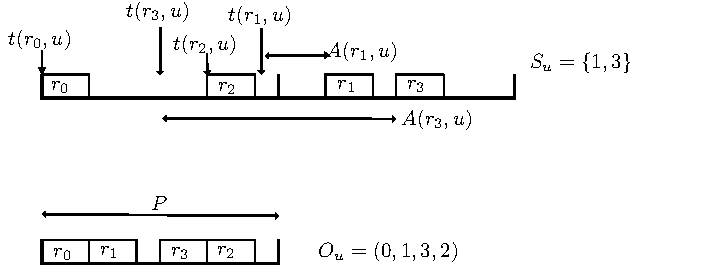
\includegraphics[scale=1]{normalizedassignment}
\caption{A compact representation of an assignment in which $O_u = (0,1,3,2)$ and $S_u = \{1,3\}$ }
\label{fig:normalizedassignment}
\end{figure}


Note that for $CR(A)$ to be defined, we need that on each contention point, a datagram is not buffered. We call such an assignment a \textbf{canonical} assignment. It turns out that any assignment $A$ can be made canonical without increasing $TR(A)$.

\begin{lemma}\label{lemma:canonical_min}
Let $A$ be a valid non canonical assignment, then there is a valid canonical assignment $A'$ such that $A' \preceq A$.
\end{lemma}
\begin{proof}
Consider a vertex $u$ of contention level $1$, such that for all $r \in \mathcal{R}_u$, $A(r,u) > 0$. Let us define $m$ as the minimimum of these values, we define $A'(r,u) = A(r,u) - m$. There are no collision on $u$, since all departure times have been translated by the same value. Moreover, if $v$ is the vertex after $u$ in a route $r$, we define  $A'(r,v) = A(r,v) + m$. Hence, all departure times for vertices of contention levels larger than one are the same in $A$ and $A'$, which implies that there are no collisions in these vertices. We have proven that $A'$ is still valid. Since all departure times of $A'$ are less or equal to those induced by $A$, we have $A' \preceq A$. Moreover, if $r_0$ is the route with $A(r_0,u) = m$, then $A'(r_0,u) = 0$. 

We apply this transformation by increasing contention level. Since, the transformation applied at some contention level do not change $A'$ for smaller contention levels, it proves that $A'$ is valid, canonical and that $A' \preceq A$.
\end{proof}


\subsection{From a compact assignment to it realization}


We now explain how to transform a compact representation into a canonical assignment.
Moreover, we will show that the obtained assignment is the smallest among all assignments of same representation. We first explain how to do the transformation on a routed network with a single contention point $u$.

Recall that the datagram of a route $r$ is available at time $t(r,u)$ in the vertex $u$.
Let us consider a compact assignment $CA$, which associates the pair $(O_u,S_u)$ to $u$.
We now define inductively how to build an assignment $Real(CA)$ from $CA$, that we call the realization of $CA$. Note that we can fail to build a realization from a compact representation, then $Real(CA)$ is undefined and we say that $CA$ is not realizable. To lighten the notation in the next paragraphs, we will denote $Real(CA)$ by $A$.

\todo{expliquer la construction avant de la faire, dans lordre croissant en terme de valeur}
Let say that the order $O_u$ is $(r_1, \dots, r_l)$. We fix $A(r_1,u)$ to zero, that is the first
datagram in the period has no buffering time. Then, in each period beginning by the first datagram, the datagrams will be in order $O_u$. Since the first datagram of the period is fixed, we use it to consider normalized arrival times and normalized sending times.
Assume that $A(r_i,u)$ have been set for $i \leq l$, we explain how to 
set $A(r_{i+1},u)$. If $r_{i+1} \notin S_u$, then we fix $A(r_{i+1},u)$ so that $ns(r_1,r_{i+1},u)$ is the maximum of $ns(r_1,r_i,u) + \tau$ and $nt(r_1,r_{i+1},u)$. If $ns(r_1,r_{i+1},u) > P - \tau$, then $CA$ is not realizable. If $r_{i+1} \in S_u$, then we fix $A(r_{i+1},u)$ so that $ns(r_1, r_{i+1},u) = ns(r_1,r_i,u) + \tau$. In both cases, if $ns(r_1, r_{i+1},u) \geq nt(r_1,r_{i+1},u)$, then $CA$ is not realizable (the sending time is in the wrong period with regard to $S_u$). 

Figure~\ref{fig:compacttoassignment} shows how an assignment $Real(CA)$ is built from a compact assignment $CA$. First, the datagram $2$ is fixed, that is, $A(r_2,u)=0$. Then, since $r_1 \in S_u$, we set $A(r_1,u)$ such that$ ns(r_2,r_1,u) = ns(r_2,r_2,u) + \tau$. Finally, since $r_0$ and $r_3 \notin S_u$, we set $A(r_0,u)$ and $A(r_3,u)$ such that $ns(r_2,r_0,u) = nt(r_2,r_0,u)$ and  $ns(r_2,r_3,u) = ns(r_2,r_0,u) + \tau$.
\begin{figure}[!h]
	\centering
	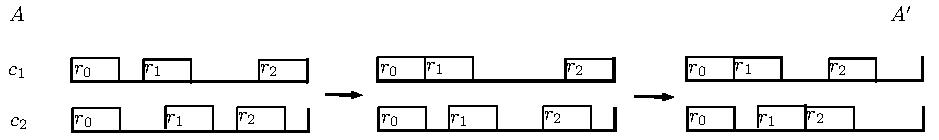
\includegraphics[scale=1]{compacttoassignment}
\caption{A canonical assignment built from a compact assignment on a signle contention point $u$. }
\label{fig:compacttoassignment}
\end{figure}

The function $Real$ can easily be generalized to any routed network. Indeed, one can first consider all vertices of contention level $1$, the routes going through them form disjoint sets. Hence, we can define $Real$ independently on each vertex of contention level $1$. 
Then using the buffering computed for this vertices, one can compute the arrival time of each route in vertices of contention level $2$ and compute $Real$ for these vertices in the exact same way, and so on for all contention levels. In the following lemmas and theorems, we always consider a single contention vertex, since it is trivial to extend any property for one contention vertex to the whole routed network as we just explained. 

\begin{lemma}\label{lemma:canonical}
The funtion $Real(CA)$ can be computed in time $O(nd)$, where $d$ is the contention
depth of the network. If $CA$ is realizable, then $Real(CA)$ is a valid canonical assignment.
\end{lemma}
\begin{proof}
In the inductive construction of $Real(CA)$,  only a constant number of comparisons and additions are needed to compute the 
the buffer time of a route from the previous one. Hence, the time spent in a vertex $u$ is linear in $|\mathcal{R}_u|$. 
A route can go through only one vertex of a given contention level, hence the time spent computing buffers for all vertices
of a contention level is in $O(n)$ and for the whole graph it is in $O(nd)$.

To prove that there are no collision between pair of routes for a given assignment, it is enough to 
prove it for any interval of time of size $P$. Hence, it is enough to consider the normalized sending time and to verify
they do not induce a collision. By construction,  $ns(r_1,r_{i+1},u)$ is always larger than $ns(r_1,r_{i},u) + \tau$ and less 
than $P - \tau$, which proves the absence of collision. Finally, $Real(CA)$ is canonical, since by definition $Real(CA)(r_1,u) = 0$,
where $r_1$ is the first route in $O_u$.
\end{proof}

We can define the following equivalence relation over canonical assignments: $A$ and $B$ are equivalent if and only if $CR(A) = CR(B)$.
We say that a compact assignment $CA = (O_u,S_u)_{u \in V(G)}$ is \emph{canonical} if it is a realizable compact assignment, $CR(Real(CA)) = (O'_u,S'_u)_{u \in V(G)}$ and if for all vertices $u$, the first route of $O_u$ and $O'_u$ coincide. This notion of canonicity is useful because the function 
$CR$ always sends a canonical assignment on a canonical compact assignment. It is just restrictive enough (by fixing the first element in each order),
that the function $CR$ is the inverse of $Real$ over canonical compact assignments. It implies that
$Real(CA)$ can be chosen as the representative of the equivalence class of the assignments having $CA$ as a representation.

In fact, as implied by the following Lemma, we can be more precise on $Real(CA)$: it is minimal in its equivalence class for $\prec$.

\begin{lemma}\label{lemma:prec}
Let $A$ be a valid assignment, then $Real(CR(A)) \preceq A$.
\end{lemma}
\begin{proof}
Given a vertex $u$ and a route $r \in \mathcal{R}_u$, we prove by induction that $Real(CR(A))(r,u) \leq A(r,u)$.
Let $(O_u,S_u)$ be the pair associated to $u$ by $CR(A)$, with $O_u = (r_1,\dots,r_l)$. By definition of $CR$, $r_1$ the first route in $O_u$, is such that $A(r_1,u) = 0$. By definition of $Real$, we have that  $Real(CR(A))(r_1,u) = 0 = A(r_1,u)$.
Now assume that $Real(CR(A))(r_i,u) \leq A(r_i,u)$ for some $i$. 

First, consider the case $r_{i+1} \notin S_u$. By definition of $CR$, $ns(r_1,r_{i+1},u)$ must be larger than 
$ns(r_1,r_{i},u)+ \tau$ and because $r_{i+1} \notin S_u$ it must also be larger than $rs(r_1,r_{i+1},u)$. 
Since $Real(CR(A))(r_{i+1},u)$ is the minimum value so that both constraints are true for $Real(CR(A))$, using
the induction hypothesis, we have $Real(CR(A))(r_i,u) \leq A(r_i,u)$. The case $r_{i+1} \in S_u$ is similar
and left to the reader.
\end{proof}


% 
% 
% Say w.l.o.g. that the datagrams are indexed in the order given by $O$.
% We fix the sending date of the first datagram $s(1) = r(1)$, that is $A(1) = 0$, the datagram does not wait in a buffer.  To simplify, we assume that $s(1) = r(1) = 0$, which can be obtained by removing $r(1)$ to all arrival times. We fix the sending date of the datagram in order, when the first $i$ datagrams have their sending date computed, we fix $s(i+1)$ in the following way. 
% 
% If $i+1 \notin S$, then $s(i+1) >= r(i+1)$ otherwise the datagram $i+1$ should go in the period after the one it is available in, that is $s(i+i) > (r(i+1)/P + 1)P$.
% The value of  $s(i+1)$ is the smallest value which satisfies the previous constraint,
% ensures that there are no collision with the first $i$ datagrams and  satisfies the order, that is $s(i+1) \mod P > s(i) \mod P$. 
% It is possible that the process fails to find a correct value for $s(i)$ at some point,
% in that case there are no assignment associated to this compact representation.
% 
% We denote this transformation by $Sol$, that is $Sol(O,S)$ is the solution previously defined
% (the routed network is implicit) or a special value to denote there is no assignment compatible with this compact representation. 
% 
% We can also define an inverse function which from most assignment $A$ computes a compact representation, that we already defined in def.~\ref{definition:compact} by $CR(A)$. The function is defined only for
% assignments $A$, such that the first datagram does not wait in a buffer, that is $s(1) = r(1)$. Assume w.l.o.g that $r(1) = s(1) = 0$, by considering the equivalent problem where $r(i)= r(i) -r(1)$ and $s(i) = s(i) - r(1)$.
% Compute the values $(s(i))\mod P$ and  call their order $O$. Let 
%  $S$ be the set of $i$ such that $(s(i) \geq (r(i) / P + 1) P$. We let $CR(A) = (O,S)$.


A compact representation of a solution for an instance of depth larger than $k$
is a list of compact representations, one for each contention arc. The following theorem explains why it is enough to explore the compact representations to solve \spall.

%\begin{theorem}
%Among all assignments $A$ for a routed network $G,{\cal R})$, there is a compact representation which minimizes $TR(A)$.
%\label{theorem:compact}
%\end{theorem}
%\begin{proof}
%Consider an assingment $A$ and a vertex $u$.
%If $A(r,u) > 0, \forall r \in {\cal R}$, it is possible to compute the assignment $A'$ such that
%$A'(r,u) = A(r,u)-\min\limits_{i \in {\cal R}} A(i,u)$. Consider a vertex $v$ such that $cl(v) = cl(u) +1$, or such that $v \in {\cal D}$ that is, $v$ comes after $u$ in any routes shared by both vertices.\\
%For all routes $r$ passing through $v$, by definition, and since $A'(r,u) \leq A(r,u)$: $$t'(r,v) = \lambda(v,r) + \sum_{u \in r, cl(u,r) < cl(v,r)} A'(r,u)  \leq t(r,v)$$\\
%Note that by reducing the buffers in a node $u_i$, we allow a datagram to reach the node $u_{i+1}$ earlier. Nevertheless, we do not change the order of the datagrams in $u_{i+1}$, even if it is possible.
%By induction, if $v$ is the last vertex of the route $r$, then : $$t'(r,v) \leq t(r,v) \implies TR(A') \leq TR(A)$$
%Thus, for all existing assignments $A$ solving \spall, it is possible to find an equivalent assignment $A'$ which have compact representation $CR(A')$ and such that $TR(A') \leq TR(A)$.\\
%\end{proof}


To solve \spall, we need to find an assignment for which $TR(A)$ is minimal. Using the previous Lemmas, it is easy to see
that it can be done by a buteforce enumeration of the compact representations, 

To do so, because of Lemma~\ref{lemma:prec}, it is enough to 
enumerate all canonical compact representation, to compute their realization and the corresponding transmission time.


%\begin{lemma}
 %The number of compact representation $(O,S)$ for a contention point with $k$ routes is $k!2^{k}$.
% \label{lemma:numberarcs}
%\end{lemma}
%\begin{proof}
%Consider the datagrams are numeroted $d_1,\ldots,d_k$.
% There is $k$ routes on the contention point. Thus, there is $k!$ possible orders for the sequence of datagram in a period.
 %Once the order $O$ of the compact representation is given, one can fix, w.l.o.g. $b(d_1) = 0$.
 %Then, there is $k-1$ remaining datagram that can be set in $S$.
 %This mean there is $k!2^{k-1}$ pairs of different $(O,S)$, i.e. compact representation for this arc.
%\end{proof}

%From lemma~\ref{lemma:numberarcs}, one can determine the numbre of compact representation of an entire routed network.
%We define $k_1,\ldots,k_l$ the number of routes on the $l$ contention points of a routed network.
%\begin{lemma}
 %The number of compact representation for a routed network $(G,{\cal R})$ is $\prod_{i=1}^l k_i!2^{k_i}$ .
 %\label{lemma:numbergraph}
%\end{lemma}

%We consider a routed network $(G,{\cal R})$. As a reminder, $CD$ is the contention depth of the routed network, and  there is $n$ routes in ${\cal R}$.
\begin{theorem}\label{theorem:FPT}
For routed networks of fixed contention depth $d$, the problem \spall parametrized by $n$ the number of routes is FPT: it can be solved in time $O(nd(n!2^{n})^{d})$.
\end{theorem}
\begin{proof}
The algorithm to solve \spall is the following: all compact assignments $CA$ are generated, for each of them $TR(Real(CA))$ is computed in time
$O(nd)$ by Lemma~\ref{lemma:canonical} and we keep the compact assignment for which this value is minimal.  Because of Lemma~\ref{lemma:prec}, to compute the minimum of $TR(A)$, it is enough 
to compute the minimum of $TR(Real(CA))$.

 Now, we need to evaluate the number of compact assignments. 
On a single contention point $u$ with $s = |\mathcal{R}_u|$ routes going through, there are $s!2^s$ possible restrictions of a compact assignment by counting the number of pairs of set and order over $\mathcal{R}_u$.
On a given contention level consisting in the vertices $\{u_1,\dots,u_l\}$, with $s_i = |\mathcal{R}_{u_{i}}|$, there are 
$\prod_{1 \leq i\leq l} s_i!2^{s_i}$. On a given contention level, all routes use at most $1$ vertex, hence $\sum_{1 \leq i\leq l} s_i \leq n$. 
By convexity of the exponential and factorial functions, we have $\prod_{1 \leq i\leq l} s_i!2^{s_i} \leq n!2^n$ and since there are $d$ contention levels,
we have at most $ (n!2^{n})^{d}$ compact assignments which proves the theorem.
\end{proof}




\section{Algorithms to solve \spall}


\subsection{Greedy Algorithm}
In order to initialize our loacal search heuristics, a compact assignment is needed. We present in this section three greedy algorithms that gives an assignment. One of them is designed to always obtain a realisable compact assignment.
\subsubsection{Greedy deadline assignment}
Here, we present a first intuitive algorithm. We want to send the datagrams as soon as they are available. If two datagrams are available at the same date, the algorithm favors the datagrams which have the most critical latency.
The contention vertices are sorted by contention level. The contention vertices of the same contention level are managed independantly. For a vertex $u$, we do the following routine:
\begin{enumerate}
\item The budget $2\times \lambda(u,r) - t(r,u)$  is computed for each routes. Note that this value can be negative since a datagram can be buffered in contention vertices before $u$.
 \item The datagram with the lowest $t(r,u)$ is sent without buffers.
 \item If one or several datagrams are available at the end of the emmision of the last datagram.
    \begin{itemize}
        \item Chose the datagram with the lowest budget, compute the delay and send it as soon as it is possible avoiding contention.
        \item Go back to step 3.
    \end{itemize}
    \item If no datagrams are available, send the one with the lowest $t(r,u)$ which have not been sent yet, as soon as it is possible, avoiding contention.
    \item Go back to step 3.
\end{enumerate}
If a datagram cannot be placed in the period because of there is no gap of $\tau$ tics between the already scheduled datagrams, the algorithms fails.
\begin{algorithm}[H]
	\caption{Greedy deadline assignment}
	\begin{algorithmic}
	\REQUIRE $(G,{\cal R})$, $P$, $\tau$
	\ENSURE An assignment $A(G,{\cal R})$, or FAILS
	\STATE $budget[|{\cal R}|]$ integer table.
	\FORALL{route $r$ in ${\cal R}$}
      \STATE  $budget[r] \leftarrow 2\times \lambda(u,r) - t(r,u)$
	\ENDFOR
	\STATE Let $first$ be the route such that $t(first,u)$ is minimal
	\STATE $A(first,u) \leftarrow 0$
	\STATE $offset \leftarrow t(first,u)+\tau$
	\STATE ${\cal R} \leftarrow {\cal R}\setminus \{first\}$
    \WHILE{ ${\cal R} \neq \emptyset$}
    \IF {$\exists i \in{\cal R}, t(i,u) \leq offset$}
    \STATE Choose $i$ with the lowest $budget[i]$
    \STATE $A(i,u) \leftarrow offset - t(i,u)$
    \STATE $offset \leftarrow offset + \tau$
    \ELSE
     \STATE Choose $i \in {\cal R}$ with the lowest $t(i,u)$
     \STATE $A(i,u) \leftarrow 0$
     \STATE $offset \leftarrow t(i,u) + \tau$
    \ENDIF
    \IF{$A$ is not valid}
    \IF{ $add\_delay \leftarrow FIRST\_VALID(A,P,i)$}
    \STATE $A(i,u) \leftarrow A(i,u) + add\_delay$
    \ELSE
   \STATE Return FAIL
    \ENDIF
    \ENDIF
    
    \ENDWHILE
    \STATE Return SUCCESS
	\end{algorithmic}
	\end{algorithm}

\todo{ajouter la routine FIRST VALID qui donne la premiere position a laquelle on peut placer le message a partir de l'offset donné}
\subsubsection{Greedy deadline Normalized}
A variant of the Greedy deadline assignment algorithm consists in choosing the datagrams by lowest normalised arrival times instead of arrival times when several datagrams are available on a given offset. In practice, it seems that this algorithm performs better.

The two previous algorithm can fail, thus, they do not give a compact assignment for all routed networks. Since a compact assignment is needed to initilize our local search algorithms, we propose a greedy algorithm that always ensure to find an assignment, even if the performances are degraded.
\subsubsection{Greedy Deadline Packed}
In order to always find an assignment with a greedy routine, we propose the following algorithm.
\begin{enumerate}
\item The budget $2\times \lambda(u,r) - t(r,u)$  is computed for each routes. Note that this value can be negative since a datagram can be buffered in contention vertices before $u$.
 \item The datagram with the lowest $t(r,u)$ is sent without buffers.
 \item The normalized arrival time is computed for each datagrams.
 \item If one or several datagrams are available at the end of the emmision of the last datagram:
    \begin{itemize}
        \item Chose the datagram with the lowest budget, compute the delay and send it as soon as it is possible avoiding contention.
        \item Go back to step 3.
    \end{itemize}
    \item If no datagrams are available, we compute for each datagram the additional latency $ad$ needed to put the datagram in second period.
    \item We take the datagram with the largest value of $budget - ad$, that is the datagram which is the less impacted beeing sent in the second period.
    \item Go back to step 3.
\end{enumerate}
\todo{Ecrire en pseudo code, utiliser les notations du papier, par exemple pour second period, dire que ca n'a pas de sens de prendre les routes non normalisés, car l'algo travaille la dessus et que de tte facon c'est meilleur pour les algos d'avant}

\subsection{Local Search Heuristics}

The number of compact representations grows extremely quickly with $n$. Hence, to find one which minimizes $TR(A)$, we propose several classical local search algorithm: hill climbing, tabu search and simulated annealing. This methods works as long as a relevant notion of neighborood of a solution is proposed. 
The neighborood relation must satisfy several properties: it must be quick to compute (hence not to large) and the implicit graph of solutions defined
by the neighborood relation should be connected. We now propose a simple neighborood relation over compact assignments.

Let $u$ be a contention vertex of a network, and let $CA$ be a compact assignment for this network, 
 which associates the pair $(O_u,S_u)$ to $u$. Let $r \in \mathcal{R}_u$, the \emph{$r$-neighborood} of $(O_u,S_u)$ is the set of pairs $(O,S)$ such that:
 
 \begin{enumerate} 
 \item $O_u = O$ or $O_u = (r_1,\dots,r_l)$ with $r_i = r$ and $O = (r_1,\dots,r_{i-2},r_{i},r_{i-1},\dots,r_{l})$ 
 \item $S_u = S \cup \{r\}$ or  $S_u = S \setminus \{r\}$ 
 \end{enumerate}

Informally, a compact representation is in the $r$-neighborood of another one if it can be obtained by 
moving down $r$ once (or not changing it) in the order and adding or removing $r$ from the set. 
Remark that the $r$-neighborood of any pair $(O_u,S_u)$ has at most $4$ members (it can be $2$ when the route $r$ is in first position and cannot be exchanged with the previous one). 

The \emph{$r$-neighborood} of a compact assignment $CA$ is the set of all compact assignments $CA'=(O'_u,S'_u)_{u \in V(G)}$, such that  $(O'_u,S'_u)$ is in the $r$-neighborood of $(O_u,S_u)$. Finally, the \emph{neighborood} of an assignment $CA$ is the union for all $r \in \cal{R}$ of the 
 $r$-neighboroods of $CA$.

% 
% 
% We define $O(r)$ the position of the route $r$ in an order $O$, and the inverse fuction $O^{-1}(r)$.\\
% We consider a compact represtation $(O_u,S_u)$ on a contention point $u$.
% A \textit{neigbhor order} of  $O$ over a route $r$, is an order $O'$ such that $O'(r) = O(r)+1$ . This means that $O'(j) = O(j),\forall j \notin \{r;O^{-1}(r)+1\}$. Indeed, by definition, $O'(O^{-1}(O(r)+1)) = O(r)$. If $r$ is the last route in the order $O$, then $O'(r) = 1$ and $O'(O^{-1}(O(1))=O(r)$
% A \textit{neigbhor subset} of $S$ over a route $r$ is defined by $S' = S - \{r\}$ if $r\in S$ or $S'= S \cup \{r\}$ if $ r \notin S$.
% The \textbf{neighborhood of the pair} $(O_u,S_u)$ ouver a route $r$ is defined by the set $N_u = \{(O_u,S_u);(O_u,S_u');(O_u',S_u);(O_u',S_u')\}$.\\
% 
% Consider a compact representation $CR(A)$ over a route $r$.
% $CR'(A)$ si a \textbf{neighbor} of $CR(A)$ if for all pair $(O_u,S_u)'$ of $CR'(A)$:
% \begin{itemize}
%  \item If $u \notin r$, $(O_u,S_u)' = (O_u,S_u)$
%  \item If $u \in r$, $(O_u,S_u)' \in N_u $
% \end{itemize}
% 
% The \textbf{neighborhood of a compact representation} $CR$ \textbf{over a route} $r$  is thus the set of compact representations: $\prod_{u\in r} N_u$.
% 
% The \textbf{\underline{neighborhood of a compact representation}} $CR$ is then the set of the compact representations over all routes, that is:
% $$ \bigcup_{r\in{\cal R}} (\prod_{u\in r} N_u ) $$.

 Let us denote by $k_1,\ldots,k_n$ the number of contention vertices on the $n$ routes of 
 a routed network $(G,\cal{R})$. Then, a compact representation has at most $\sum_{i=1}^n 4^{k_i}$ neighbors. Since we always work with networks of bounded contention depth ($2$ or $3$ in practice), the size of a neighborhood is linear in the number of routes.
 Remark that, with this definition, we allow to include unrealizable compact assignment in a neighborood. We can easily forbid them and we will, since it is much more practical for several of our algorithms. 
 \todo{Expliquer que le graphe des solutions réalisable est connexe (il suffit d'utiliser des datagrams en position 2, les bouger ne peut pas rendre la soluce non réalisable)}
 
\subsection{Branch and Bound}
We define a \textbf{partial compact representation} $Pcr$ of a routed network $(G,R)$ as a choice of pairs $(O,S)$ on a subset of the arcs of the graph.
The function $Bound(Pcr)$ gives a lower bound of $TR(G,{\cal R})$, considering Pcr.


 As explained on theroem~\ref{theorem:compact} there is a compact representation which minimizes $TR(G,{\cal R})$. We browse the entire set of compact representation to find the one which minimizes $TR(G,{\cal R})$.\\
 To do so, we design the following branch and bound algorithm. First, we determine an upper bound for our branch and bound algorithm by computing $TR(G,{\cal R})$ with a greed algorithm. Then, for all arcs (sorted by contention level), we enumerate all the possible compact representations. For each of those compact representation, we compute $Bound(Pcr)$. If the result given by this function is higher than the upper bound already found, we do no consider this compact representation. Otherwise, we go to the next arc. Once we have chose an pair $(O,S)$ for all arcs, we compute $Sol(O,S)$ for all arcs, and if the given $TR(G,{\cal R})$ is lower than the previous upper bound we update this value for the rest of the search.\\


In order to speed up the search, we made the following cuts:

définition des différentes coupes.\\

\section{Results}




\subsection{Random generation of routed network}
Dans le cas d'application C-RAN, on prends un nombre de routes limitées (<20) et des tailles de routes petites. Néanmoins, on regarde des instances pour lesquelles le problème est difficile.\

Définition du type de graph regardés, expliquer que les instances sont plus dures quand les routes sont de tailles similaires et quand on augmente le nombre de points de contentions.\\

\subsection{Neighborood heuristics}

Étudier empiriquement les différentes variantes, paramètres, solution de départ, cout en temps ...


Taboo : Avec une hash table pour la mémoire, ce qui rend long la recherche quand on fait beaucoup de pas\\

Recuit, expliquer comment j'ai réglé la température etc\\


\subsection{Branch and bound}

Montrer avec des courbes (nombre de représentation générées et pourcentage de minimales en fonction du nombre de routes) que ces coupes sont très efficace, elles permettent de générer uniquement des représentations compactes canoniques, et presque aucunes dont la réalisation n'est pas minimale.
très peu de représentation compacte en  



\subsection{Results comparison}

\section{Conclusion}
C'est vraiment génial comme travail, on va tuer le game du DETNET.

\bibliographystyle{ieeetr}
\bibliography{srcs}
\end{document}
